\documentclass[aspectratio=169]{beamer}
\usetheme{Madrid}
\usecolortheme{whale}

\usepackage[utf8]{vietnam}
\usepackage{tikz}
\usepackage{amsmath}
\usetikzlibrary{arrows.meta,positioning}

\title{Thuật toán Dijkstra}
\subtitle{Tìm đường đi ngắn nhất trên đồ thị}
\author{Nhóm 7}
\date{\today}

\begin{document}

%================================================
\begin{frame}
\titlepage
\end{frame}

%================================================
\begin{frame}{Nội dung}
\tableofcontents
\end{frame}

%================================================
\section{Bài toán}

%------------------------------------------------
\begin{frame}{Bài toán đặt ra}

\begin{block}{Input}
Đồ thị có trọng số không âm
\end{block}

\begin{block}{Yêu cầu}
Tìm khoảng cách ngắn nhất từ đỉnh nguồn $s$ đến mọi đỉnh còn lại
\end{block}

\begin{block}{Ứng dụng}
\begin{itemize}
\item Bản đồ \& GPS
\item Mạng máy tính
\item Tối ưu chi phí vận chuyển
\end{itemize}
\end{block}

\end{frame}

%================================================
\section{Ý tưởng thuật toán}

%------------------------------------------------
\begin{frame}{Ý tưởng tham lam}

\begin{itemize}
\item Luôn chọn đỉnh chưa xét có khoảng cách nhỏ nhất
\item Cố định khoảng cách của đỉnh đó
\item Cập nhật (relax) các đỉnh kề
\item Lặp lại cho đến khi duyệt hết
\end{itemize}

\begin{block}{Tư tưởng chính}
Mở rộng dần vùng tối ưu từ đỉnh nguồn
\end{block}

\end{frame}

%------------------------------------------------
\begin{frame}{Các bước chính}

\begin{enumerate}
\item Khởi tạo:
\[
dist[s] = 0,\quad dist[v] = \infty
\]

\item Đưa $(0,s)$ vào priority queue

\item Lặp:
\begin{itemize}
\item Lấy đỉnh có dist nhỏ nhất
\item Relax các cạnh kề
\end{itemize}

\item Kết thúc khi hàng đợi rỗng
\end{enumerate}

\end{frame}

%================================================
\section{Cấu trúc dữ liệu}

%------------------------------------------------
\begin{frame}{Cấu trúc cần dùng}

\begin{itemize}
\item Danh sách kề lưu đồ thị
\item Mảng $dist[]$ lưu khoảng cách ngắn nhất
\item Priority queue chọn đỉnh gần nhất
\item Mảng $visited[]$ (tuỳ chọn)
\end{itemize}

\begin{block}{Tối ưu quan trọng}
Dùng heap để giảm độ phức tạp
\end{block}

\end{frame}

%================================================
\section{Code thuật toán}

%------------------------------------------------
\begin{frame}[fragile]{Code Dijkstra}

\begin{center}
\includegraphics[height=0.9\textheight]{Code_dijkstra.png}
\end{center}

\end{frame}

%================================================
%------------------------------------------------
\begin{frame}{Mô phỏng Dijkstra}

\begin{center}
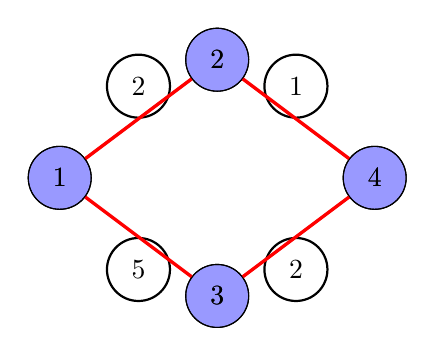
\begin{tikzpicture}[
scale=1,
every node/.style={circle,draw,minimum size=8mm},
edge/.style={draw,thick},
sel/.style={fill=blue!40},
relax/.style={draw=red,very thick}
]

% Nodes
\node<1->[sel] (1) at (0,0) {1};
\node<2->[sel] (2) at (2,1.5) {2};
\node<3->[sel] (4) at (4,0) {4};
\node<4->[sel] (3) at (2,-1.5) {3};

\node<1->[circle,draw] (1a) at (0,0) {1};
\node<1->[circle,draw] (2a) at (2,1.5) {2};
\node<1->[circle,draw] (3a) at (2,-1.5) {3};
\node<1->[circle,draw] (4a) at (4,0) {4};

% Edges base
\draw[edge] (1a)-- node[above]{2} (2a);
\draw[edge] (1a)-- node[below]{5} (3a);
\draw[edge] (2a)-- node[above]{1} (4a);
\draw[edge] (3a)-- node[below]{2} (4a);

% Relax highlights
\draw<2->[relax] (1a)--(2a);
\draw<2->[relax] (1a)--(3a);
\draw<3->[relax] (2a)--(4a);
\draw<4->[relax] (4a)--(3a);

\end{tikzpicture}
\end{center}

\vspace{6pt}

\small
\begin{itemize}
\item<1-> Bước 1: Chọn đỉnh nguồn 1, $dist[1]=0$
\item<2-> Bước 2: Relax cạnh $(1\to2),(1\to3)$  
\quad $dist[2]=2,\ dist[3]=5$
\item<3-> Bước 3: Chọn đỉnh 2 (nhỏ nhất), relax $(2\to4)$  
\quad $dist[4]=3$
\item<4-> Bước 4: Chọn đỉnh 4, relax $(4\to3)$  
\quad Không cải thiện
\end{itemize}

\end{frame}
%================================================
\section{Độ phức tạp}

%------------------------------------------------
\begin{frame}{Phân tích độ phức tạp}

\begin{block}{Dùng mảng thường}
$O(V^2)$
\end{block}

\begin{block}{Dùng Priority Queue (Heap)}
$O((V+E)\log V)$
\end{block}

\begin{block}{Thực tế}
Rất nhanh với đồ thị thưa
\end{block}

\end{frame}

%================================================
\section{So sánh thuật toán}

%------------------------------------------------
\begin{frame}{So sánh với thuật toán khác}

\small
\begin{center}
\begin{tabular}{c|c|c}
Thuật toán & Trọng số âm & Độ phức tạp \\
\hline
BFS & Không & $O(V+E)$ \\
Dijkstra & Không & $O((V+E)\log V)$ \\
Bellman--Ford & Có & $O(VE)$ \\
Floyd--Warshall & Có & $O(V^3)$ \\
\end{tabular}
\end{center}

\end{frame}

%================================================
\section{Kết luận}

%------------------------------------------------
\begin{frame}{Tổng kết}

\begin{itemize}
\item Dijkstra tìm đường đi ngắn nhất hiệu quả
\item Áp dụng cho đồ thị trọng số không âm
\item Cốt lõi: tham lam + heap
\item Nền tảng cho nhiều bài toán tối ưu
\end{itemize}

\end{frame}

%------------------------------------------------
\begin{frame}
\centering
\Huge
Cảm ơn các bạn đã lắng nghe!
\end{frame}

%================================================
\end{document}